\documentclass[11pt]{article} 
\usepackage[english]{babel}
\usepackage[utf8]{inputenc}
\usepackage[margin=0.5in]{geometry}
\usepackage{amsmath}
\usepackage{amsthm}
\usepackage{amsfonts}
\usepackage{amssymb}
\usepackage[usenames,dvipsnames]{xcolor}
\usepackage{graphicx}
\usepackage[siunitx]{circuitikz}
\usepackage{tikz}
\usepackage[colorinlistoftodos, color=orange!50]{todonotes}
\usepackage{hyperref}
\usepackage[numbers, square]{natbib}
\usepackage{fancybox}
\usepackage{epsfig}
\usepackage{soul}
\usepackage[framemethod=tikz]{mdframed}
\usepackage[shortlabels]{enumitem}
\usepackage[version=4]{mhchem}
\usepackage{multicol}
\usepackage{forest}
\usepackage{mathtools}
\usepackage{comment}
\usepackage{enumitem}
\usepackage[utf8]{inputenc}
\usepackage[linesnumbered,ruled,vlined]{algorithm2e}
\usepackage{listings}
\usepackage{color}
\usepackage[numbers]{natbib}
\usepackage{subfiles}
\usepackage{tkz-berge}


\newtheorem{prop}{Proposition}[section]
\newtheorem{thm}{Theorem}[section]
\newtheorem{lemma}{Lemma}[section]
\newtheorem{cor}{Corollary}[prop]

\theoremstyle{definition}
\newtheorem{definition}{Definition}

\theoremstyle{definition}
\newtheorem{required}{Problem}

\theoremstyle{definition}
\newtheorem{ex}{Example}


\setlength{\marginparwidth}{3.4cm}
%#########################################################

%To use symbols for footnotes
\renewcommand*{\thefootnote}{\fnsymbol{footnote}}
%To change footnotes back to numbers uncomment the following line
%\renewcommand*{\thefootnote}{\arabic{footnote}}

% Enable this command to adjust line spacing for inline math equations.
% \everymath{\displaystyle}

% _______ _____ _______ _      ______ 
%|__   __|_   _|__   __| |    |  ____|
%   | |    | |    | |  | |    | |__   
%   | |    | |    | |  | |    |  __|  
%   | |   _| |_   | |  | |____| |____ 
%   |_|  |_____|  |_|  |______|______|
%%%%%%%%%%%%%%%%%%%%%%%%%%%%%%%%%%%%%%%

\title{
\normalfont \normalsize 
\textsc{CSCI 3104 Spring 2022 \\ 
Instructors: Profs. Chen and Layer} \\
[10pt] 
\rule{\linewidth}{0.5pt} \\[6pt] 
\huge Problem Set 0 \\
\rule{\linewidth}{2pt}  \\[10pt]
}
%\author{}
\date{}

\begin{document}

\maketitle


%%%%%%%%%%%%%%%%%%%%%%%%%
%%%%%%%%%%%%%%%%%%%%%%%%%%
%%%%%%%%%%FILL IN YOUR NAME%%%%%%%
%%%%%%%%%%AND STUDENT ID%%%%%%%%
%%%%%%%%%%%%%%%%%%%%%%%%%%
\noindent
Due Date \dotfill January 18, 2022 \\
Name \dotfill \textbf{Julia Troni} \\
Student ID \dotfill \textbf{109280095} \\
Collaborators \dotfill \textbf{My own brain}

\tableofcontents

\section{Instructions}
 \begin{itemize}
	\item The solutions \textbf{should be typed}, using proper mathematical notation. We cannot accept hand-written solutions. \href{http://ece.uprm.edu/~caceros/latex/introduction.pdf}{Here's a short intro to \LaTeX.}
	\item You should submit your work through the \textbf{class Canvas page} only. Please submit one PDF file, compiled using this \LaTeX \ template.
	\item You may not need a full page for your solutions; pagebreaks are there to help Gradescope automatically find where each problem is. Even if you do not attempt every problem, please submit this document with no fewer pages than the blank template (or Gradescope has issues with it).

	\item You are welcome and encouraged to collaborate with your classmates, as well as consult outside resources. You must \textbf{cite your sources in this document.} \textbf{Copying from any source is an Honor Code violation. Furthermore, all submissions must be in your own words and reflect your understanding of the material.} If there is any confusion about this policy, it is your responsibility to clarify before the due date. 

	\item Posting to \textbf{any} service including, but not limited to Chegg, Reddit, StackExchange, etc., for help on an assignment is a violation of the Honor Code.

	\item You \textbf{must} virtually sign the Honor Code (see Section \ref{HonorCode}). Failure to do so will result in your assignment not being graded.
\end{itemize}


\section{Honor Code (Make Sure to Virtually Sign)} \label{HonorCode}

\begin{required}
\begin{itemize}
\item My submission is in my own words and reflects my understanding of the material.
\item Any collaborations and external sources have been clearly cited in this document.
\item I have not posted to external services including, but not limited to Chegg, Reddit, StackExchange, etc.
\item I have neither copied nor provided others solutions they can copy.
\end{itemize}

%\noindent In the specified region below, clearly indicate that you have upheld the Honor Code. Then type your name. 
\end{required}

\begin{proof}[I agree to the above, Julia Troni.]
%% Typing "I agree to the above," followed by your name is sufficient.
\end{proof}


\newpage
\section{\LaTeX\ Intro}

\subsection{Problem \ref{Latex1}}
\begin{required} \label{Latex1}
By default, text in \LaTeX\ is represented as normal text. To write math, we put it between \$ signs, which is called math mode.
This equation is in math mode: $E=mc^2$.

Please recreate the following image using \LaTeX:

\fbox{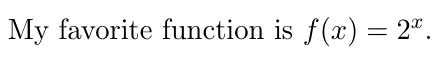
\includegraphics[width=0.3\textwidth]{task1}}
\end{required}

\begin{proof}[Answer]
%Your answer goes here

My favorite function is $f(x)= 2^{x}$
\end{proof}



\newpage
\subsection{Problem \ref{Latex2}} 
\begin{required} \label{Latex2}
Commands are prefaced by a backslash, for example, in math mode, the command \texttt{\textbackslash theta} creates the Greek letter theta, i.e. $\theta$.

Curly braces are used to group symbols together. For example, to write $2^{a + b}$, we write \texttt{2\^{}\{a + b\}}.

Please recreate the following image using \LaTeX:

\fbox{
\includegraphics[width=0.3\textwidth]{task2}}
\end{required}

\begin{proof}
%Your answer goes here.

Did you know that $e^{\pi i}= -1$?
\end{proof}



\newpage
\subsection{Problem \ref{Latex3}}
\begin{required} \label{Latex3}
Some commands take one or more arguments, which go in curly braces immediately after the commands. For example, the command \texttt{\textbackslash textbf} takes one argument and makes \textbf{text bold}.

In math mode, the command \texttt{\textbackslash sqrt} takes one argument and places the square-root symbol around it. The \texttt{\textbackslash frac} command takes two arguments, a numerator and a denominator, and creates a fraction.

Please recreate the following image using \LaTeX:

\fbox{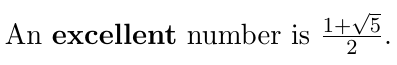
\includegraphics[width=0.3\textwidth]{task3}}
\end{required}

\begin{proof}
%Your answer goes here.
An \textbf{excellent} number is $\frac{1+\sqrt{5}}{2}$.
\end{proof}



\newpage
\subsection{Problem \ref{Latex4}}
\begin{required} \label{Latex4}
To write math over multiple lines, we can use the align environment.
It can be used as follows:
\begin{verbatim}
\begin{align*}
  16 &= 4 \cdot 4      \\
     &= 2^2 \cdot 2^2  \\
     &= 2^4 .
\end{align*}
\end{verbatim}
This produces:
\begin{align*}
  16 &= 4 \cdot 4      \\
     &= 2^2 \cdot 2^2  \\
     &= 2^4 .
\end{align*}
The ampersand specifies where to align each row with the row above. The double-backslash creates a break to a new line.

Please recreate the following image using \LaTeX (hint: use the command \texttt{\textbackslash log}):

\begin{center}
\fbox{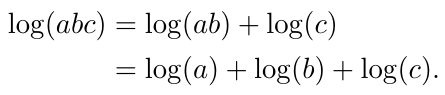
\includegraphics[width=0.3\textwidth]{task4}}
\end{center}
\end{required}

\begin{proof}
%Your answer goes here.

\begin{align*}
\log(abc) &= \log(ab) + \log(c) \\
 &= \log(a) + \log(b) + \log(c).
\end{align*}


\end{proof}



%%%%%%%%%%%%%%%%%%%%%%%%%%%%%%%%%%%%%%%%%%%%%%%%%%

\end{document} % NOTHING AFTER THIS LINE IS PART OF THE DOCUMENT



